\documentclass[a4paper]{article} % Specify A4 paper

% Optional packages
\usepackage[utf8]{inputenc} % Allows UTF-8 input
\usepackage[T1]{fontenc}    % Selects font encodings
\usepackage{amsmath}        % For mathematical formulas
\usepackage{graphicx}       % To include images
\usepackage[ngerman]{babel} % German language support
\usepackage{geometry}       % For page layout adjustments
\usepackage{lipsum}         % For generating dummy text to fill pages
\usepackage{blindtext}      % Another package for dummy text

% Adjust page margins if needed (optional, default article margins are usually fine)
% \geometry{a4paper, margin=2.5cm}

% Document information
\title{Dokumentation zur Pipeline-Architektur}
\author{Ihr Name / Projektgruppe}
\date{\today}

\begin{document}

\section{Praktische Umsetzung: Beispiel einer Datenverarbeitungs-Pipeline}
\subsection{Gesamtarchitektur}
Im folgenden Beispiel soll auf Basis der Pipeline-Architektur eine einfache Datenverarbeitungs-Pipeline beschrieben werden. Mit dieser Pipeline sollen Sensordaten geladen, verarbeitet und gespeichert werden. Die Pipeline besteht dabei aus mehreren Segmenten wobei der Ladepunkt der Datei als Startpunkt dient.
Die Architektur ist in Abbildung \ref{fig:architektur} dargestellt. Die einzelnen Stufen sind in der Abbildung nummeriert.
Die Pipeline besteht aus den folgenden Stufen:
\begin{enumerate}
    \item \textbf{Datenerfassung:} Sammeln von Rohdaten von Sensoren.
    \item \textbf{Vorverarbeitung:} Bereinigen und Filtern der Rohdaten.
    \item \textbf{Anreicherung:} Hinzufügen von Kontextinformationen (z.B. Zeitstempel, Standort).
    \item \textbf{Analyse:} Durchführung spezifischer Berechnungen oder Mustererkennung.
    \item \textbf{Speicherung/Ausgabe:} Persistieren der Ergebnisse oder Weiterleitung an andere Systeme.
\end{enumerate}

\subsection{Implementierung der Pipeline-Steuerung: Die Wrapper-Klasse}
Nachdem die grundlegende Architektur und die einzelnen Stufen definiert sind, bedarf es einer Komponente, welche die Pipeline als Ganzes verwaltet und deren Ausführung steuert. Hierfür gibt es verschiedene Ansätze:

\begin{itemize}
    \item \textbf{Direkte Implementierung im Code:} Die Abfolge der Stufen wird direkt im ausführenden Code definiert. Dies ist einfach für kleine Pipelines, kann aber bei wachsender Komplexität unübersichtlich und schwer wartbar werden.
    \item \textbf{Konfigurationsbasierter Ansatz:} Die Pipeline-Struktur wird in einer externen Datei (z.B. YAML, JSON) definiert und zur Laufzeit geladen. Dies bietet hohe Flexibilität und ermöglicht Anpassungen ohne Code-Änderungen, erfordert jedoch zusätzlichen Aufwand für das Parsen und Validieren der Konfiguration.
    \item \textbf{Wrapper-Klasse:} Eine dedizierte Klasse kapselt die Logik zur Verwaltung der Stufen (Hinzufügen, Reihenfolge) und zur Ausführung der Pipeline. Dies fördert die Struktur, Kapselung und Wiederverwendbarkeit.
\end{itemize}

Für dieses Beispiel wird der Ansatz der Wrapper-Klasse gewählt, da er eine gute Balance zwischen Struktur, Flexibilität und Implementierungsaufwand bietet. Die Kernidee ist eine Klasse (z.B. `Pipeline`), die eine Liste von Pipeline-Stufen verwaltet und eine Methode zur Ausführung der gesamten Sequenz bereitstellt. Abbildung \ref{fig:wrapper} zeigt ein Klassendiagramm für eine solche Wrapper-Klasse.

\begin{figure}[htbp]
    \centering
    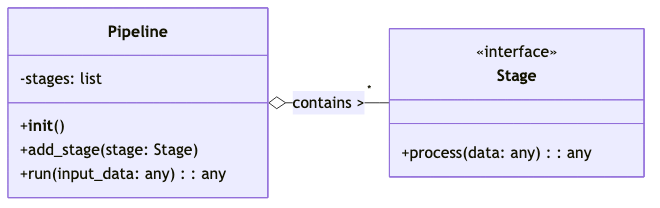
\includegraphics[width=0.8\textwidth]{img/wrapper.png}
    \caption{Klassendiagramm der Pipeline Wrapper-Klasse (`Pipeline`) und der abstrakten Stufenklasse (`Stage`).}
    \label{fig:wrapper}
\end{figure}

Die `Pipeline`-Klasse könnte typischerweise Methoden wie `\_\_init\_\_` (zur Initialisierung, z.B. einer leeren Liste für die Stufen), `add\_stage` (zum Hinzufügen einer Stufe zur Pipeline) und `execute` oder `run` (zum Durchlaufen aller Stufen mit den Eingabedaten) besitzen.

Ein zentrales Element dieses Ansatzes ist die Verwendung einer abstrakten Basisklasse oder einer Schnittstelle für die einzelnen Pipeline-Stufen (im Diagramm und folgenden Codebeispiel als `Stage` bezeichnet). Jede konkrete Stufe (wie Datenerfassung, Vorverarbeitung etc.) muss von dieser Basisklasse erben und deren definierte Methoden (z.B. eine `process` oder `execute`-Methode) implementieren. Dies stellt sicher, dass alle Stufen einheitlich behandelt und von der `Pipeline`-Klasse aufgerufen werden können.

Die Wrapper-Klasse kann zudem sicherstellen, dass nur valide Stufen hinzugefügt werden. Dies wird oft durch Typ-Prüfungen realisiert, wie im folgenden Python-Codeausschnitt für die `add_stage`-Methode gezeigt\:

\begin{verbatim}
# Innerhalb der Pipeline-Wrapper-Klasse
def add_stage(self, stage: Stage):
    """Fügt eine neue Stufe zur Pipeline hinzu."""
    if not isinstance(stage, Stage): # Prüft, ob das Objekt eine Instanz von Stage oder einer Subklasse ist
        raise TypeError("Übergebene Stufe muss eine Instanz von Stage sein.")
    self.stages.append(stage) # Annahme: self.stages ist die Liste der Stufen
\end{verbatim}

Diese Prüfung mittels `isinstance(stage, Stage)` stellt sicher, dass jedes Objekt, das der Pipeline hinzugefügt wird, tatsächlich vom Typ `Stage` (oder einer davon abgeleiteten Klasse) ist und somit die erwartete Schnittstelle (z.B. eine `process`-Methode) implementiert. Wird ein unpassendes Objekt übergeben, wird ein `TypeError` ausgelöst, was die Robustheit der Pipeline erhöht.

Die Kapselung der Pipeline-Logik in einer Wrapper-Klasse in Kombination mit einer abstrakten Basisklasse für die Stufen führt zu einem modularen, gut testbaren und erweiterbaren Design. Änderungen an einzelnen Stufen oder das Hinzufügen neuer Stufen beeinflussen die Wrapper-Klasse nur minimal, solange die definierte Schnittstelle eingehalten wird.

\begin{verbatim}
def add_stage(self, stage:Stage):
    if(not issubclass(stage, Stage)):
        raise TypeError("stage must be an instance of Stage")
\end{verbatim}\

Diese Sicherung wird in Python durch das Prüfen des Klassentyps (issubclass) sichergestellt. Wird eine Klasse übergeben welche keine Subklasse von Stage ist wird ein TypeError geworfen. Dies geschieht bei issubclass selbst bei einer erzeugten Instanz von Stage selbst.

\subsection{Factory Pattern zur dynamischen Komponentenauswahl}
Ein weiteres nützliches Entwurfsmuster, das häufig in Verbindung mit der Pipeline-Architektur eingesetzt wird, ist das Factory Pattern. Dieses Muster gehört zu den Erzeugungsmustern und dient dazu, Objekte zu erstellen, ohne die genaue Klasse des zu erstellenden Objekts im Voraus festlegen zu müssen. Stattdessen wird die Verantwortung für die Objekterzeugung an eine spezialisierte "Factory"-Klasse oder -Methode delegiert.

Das Factory Pattern ermöglicht eine signifikante Entkoppelung des aufrufenden Codes (in unserem Fall die Pipeline oder eine ihrer Stufen) von der konkreten Implementierung der zu erzeugenden Objekte. Die Factory fungiert als zentraler Punkt für die Erzeugung von Objekten eines bestimmten Typs oder einer bestimmten Schnittstelle. Abhängig von den übergebenen Parametern oder dem Kontext entscheidet die Factory, welche spezifische Unterklasse instanziiert und zurückgegeben werden soll.

\subsubsection{Anwendung im Datenlader}
In unserem Beispiel einer Datenverarbeitungs-Pipeline findet das Factory Pattern eine praktische Anwendung, insbesondere bei der Funktion zum Auslesen der Sensordateien. Unterschiedliche Sensoren oder Datenquellen können ihre Daten in verschiedenen Formaten bereitstellen (z.B. CSV, JSON, XML, Binärformate). Anstatt die Logik zur Erkennung und Verarbeitung jedes Formats direkt in die Pipeline-Stufe einzubetten, die die Daten lädt, wird eine `LoaderFactory` eingesetzt.

Der Ablauf ist typischerweise wie folgt:
\begin{enumerate}
    \item Eine vorherige Pipeline-Stufe oder der Initialaufruf übergibt den Dateipfad oder eine andere Kennung der zu ladenden Daten an die Stufe, die für das Laden zuständig ist.
    \item Diese Ladestufe delegiert die Erzeugung des passenden Ladeobjekts an die `LoaderFactory`. Sie übergibt dabei relevante Informationen, wie z.B. den Dateipfad oder explizit das Dateiformat.
    \item Die `LoaderFactory` analysiert die übergebenen Informationen (z.B. die Dateiendung wie `.csv` oder `.json`).
    \item Basierend auf dieser Analyse instanziiert die Factory ein konkretes Ladeobjekt (z.B. eine Instanz von `CsvLoader` oder `JsonLoader`), das eine gemeinsame Schnittstelle (z.B. `DataLoader`) implementiert.
    \item Die Factory gibt das erzeugte Ladeobjekt an die aufrufende Pipeline-Stufe zurück.
    \item Die Pipeline-Stufe verwendet nun das erhaltene Ladeobjekt, um die Daten zu laden, ohne die spezifische Implementierung des Laders kennen zu müssen. Sie interagiert nur über die definierte Schnittstelle (`DataLoader`).
\end{enumerate}

Abbildung \ref{fig:loaderFactory} illustriert diesen Entscheidungsprozess innerhalb der Factory. Die Factory prüft das angeforderte Format und wählt den entsprechenden Loader aus. Sollte kein passender Loader für das angeforderte Format registriert sein oder die Datei nicht existieren, wird typischerweise ein Fehler ausgelöst oder ein Null-Objekt zurückgegeben, um das Problem zu signalisieren.

\begin{figure}[htbp] % h: here, t: top, b: bottom, p: page of floats
    \centering % Center the image
    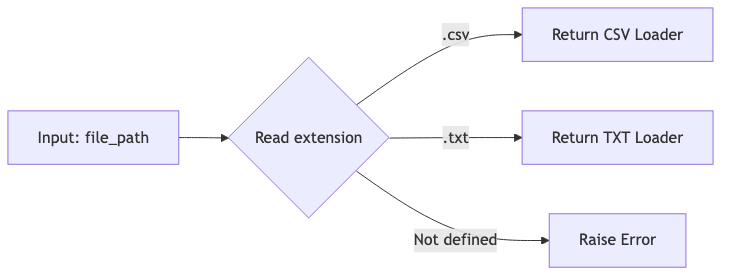
\includegraphics[width=0.8\textwidth]{img/LoaderFactory.png} % Include the image, adjust width as needed
    \caption{Entscheidungsdiagramm der LoaderFactory zur Auswahl des passenden Datenladers basierend auf dem Dateiformat.} % Add a caption
    \label{fig:loaderFactory} % Add a label for referencing
\end{figure}

\subsubsection{Vorteile des Factory Patterns in der Pipeline}
Der Einsatz des Factory Patterns in diesem Kontext bietet mehrere signifikante Vorteile:

\begin{itemize}
    \item \textbf{Entkoppelung:} Der Code der Pipeline-Stufe, die Daten lädt, ist von den konkreten Ladeimplementierungen entkoppelt. Er interagiert nur mit der Factory und der abstrakten `DataLoader`-Schnittstelle.
    \item \textbf{Flexibilität und Erweiterbarkeit (Open/Closed Principle):} Das Hinzufügen der Unterstützung für neue Dateiformate wird erheblich vereinfacht. Es muss lediglich eine neue `DataLoader`-Unterklasse (z.B. `XmlLoader`) implementiert und die `LoaderFactory` entsprechend erweitert werden, um diese neue Klasse bei Bedarf zu instanziieren. Der Code der Pipeline-Stufe selbst muss nicht modifiziert werden. Das System ist offen für Erweiterungen, aber geschlossen für Modifikationen.
    \item \textbf{Zentralisierung der Erzeugungslogik:} Die Logik zur Entscheidung, welcher Loader wann erstellt wird, ist an einem einzigen Ort – der Factory – konzentriert. Dies verbessert die Wartbarkeit und Übersichtlichkeit des Codes. Änderungen an der Erzeugungslogik müssen nur an dieser zentralen Stelle vorgenommen werden.
    \item \textbf{Verbesserte Testbarkeit:} Die einzelnen Loader-Klassen sowie die Factory selbst können isoliert getestet werden.
    \item \textbf{Wiederverwendbarkeit:} Die Factory und die Loader-Klassen können potenziell auch in anderen Teilen der Anwendung oder in anderen Projekten wiederverwendet werden. Wie bereits erwähnt, ist dies besonders nützlich, wenn die Ladefunktionalität als Teil eines wiederverwendbaren Moduls, Plugins oder Pakets (Pip Package) bereitgestellt wird. Entwickler, die das Paket nutzen, können eigene Loader hinzufügen und über die Factory registrieren (falls die Factory dies unterstützt), ohne den Kerncode des Pakets ändern zu müssen.
\end{itemize}

Zusammenfassend lässt sich sagen, dass das Factory Pattern die Struktur der Pipeline verbessert, indem es die Erzeugung von Komponenten wie Datenladern flexibler, wartbarer und erweiterbarer gestaltet. Es fördert ein sauberes Design, indem es Abhängigkeiten reduziert und Verantwortlichkeiten klar trennt.


\end{document}